\chapter{Related Work}
\label{chap:Related Work}

Before we can start to investigate the usage of machine-learning based interpolation techniques in the context of urban climate data, we first need to understand what UHIs are and how they can be classified and detected in order to define requirements for the ML models later on. Especially in the context of smart cities with new possibilities such as sensor networks, we need to understand how urban climate data can be collected and what challenges arise such as spatial and temporal data availability, data quality and more. Due to the complexity of the urban climate~\cite{oke2006guideline}, special domain knowledge is needed to understand the data and the underlying processes.
Finally, we need to get an understanding of existing interpolation techniques, traditionally in the form of regression analyses or in the context of climate data, geostatistical models, in order to define a baseline for the evaluation of ML-based models.

\section{Urban Heat Islands (UHI)}

UHIs have been the center of a lot of attention for quite some time in the scientific community. As early as 1833, with the research of Luke Howard in London which observed higher temperatures inside London than in surrounding areas~\cite{howard1833climate}, UHIs have seen a steadily increase in scientific contributions. The term \textit{Urban Heat Island} was first introduced in the 1940s~\cite{balchin1947micro}. The recording and investigation of UHIs has seen mayor steps since the begin of modern climatology, also known as the Sundborg's era beginning with Sundborg's 1951 classic heat island study of Uppsala~\cite{sundborg1951climatological}. UHIs occur in many cities around the globe~\cite{peng2012surface} in different climatic zones, during different times of day and in different intensities.\\
UHIs are so important, because heat related deaths are rising across the globe~\cite{kovats2008heat} and extreme heat waves are projected to occur more often and extreme with the ongoing climate change~\cite{lorenz2019detection}. Heat also has significant impact on human performance~\cite{kjellstrom2016heat}, mental health~\cite{obradovich2018empirical}, or might disrupt sleep~\cite{obradovich2017nighttime} and causes other issues such as overheating that causes urban infrastrcuture to fail, decreased air quality and low outdoor thermal comfort levels~\cite{stone2013climate}.

\subsection{UHI Classification}

UHIs can be classified in many different ways. Typically, there is a horizontal classification, defining the superficial extension of the UHI from micro-, to local- to meso-scale, and a vertical classification, defining in which vertical layer of the urban area the heat island is observed. To better understand these scales and the anatomy of the planitory/urban boundary layer, figures \ref{fig:mesoscale boundary layer}, \ref{fig:localscale boundary layer}, and \ref{fig:microscale boundary layer} show a detailed view of the meso-, local- and micro-scale of the urban climate respectively, as illustrated by Oke 2006~\cite{oke2006guideline}.

\begin{figure}[h]
    \centering
    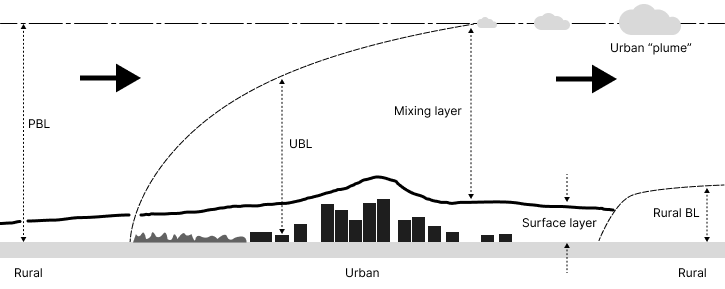
\includegraphics[width=\textwidth]{images/Mesoscale Boundary Layer.png}
    \caption{Mesoscale view of the urban climate, redrawn from~\cite{oke2006guideline}}
    \label{fig:mesoscale boundary layer}
\end{figure}

The mesoscale, as depicted in Fig~\ref{fig:mesoscale boundary layer}, spans the whole urban environment of a city, typically tens of kilometres. There are several boundary layers, that comprise different scales. The planetary boundary layer (PBL)~\cite{wyngaard1985structure} is the lowest layer of the Earth's atmosphere and spans from the surface to a height of several hundred meters up to several kilometers. It is characterised by the turbulent mixing of air, forming wind currents, that are mayorly influenced by the underlying surface.

\begin{figure}[h]
    \centering
    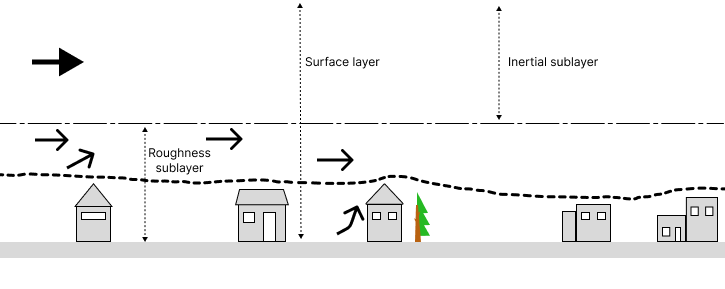
\includegraphics[width=\textwidth]{images/Localscale Boundary Layer.png}
    \caption{Localscale view of the urban climate, redrawn from~\cite{oke2006guideline}, (Todo finish)}
    \label{fig:localscale boundary layer}
\end{figure}

The localscale is situated closer to the surface and contains landscape features such as topography, but does not yet include microscale effects. At this layer, the underlying microclimatic effects in form of fluxes mix together to form a more average and representative view of the source area, typically at the scale of one to several kilometers. This layer is monitored by weather stations that are located at/or sligthly above the canopy height.

\begin{figure}[h]
    \centering
    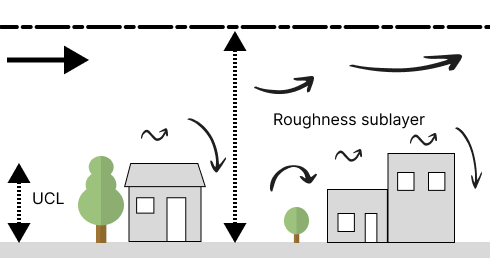
\includegraphics[width=\textwidth]{images/microscale boundary layer.png}
    \caption{Microscale view of the urban climate, redrawn from~\cite{oke2006guideline}, (Todo)}
    \label{fig:microscale boundary layer}
\end{figure}

The microscale usually ranges from a neighborhood scale to individual street canyons or even microclimates created by individual buildings. It is mayorly influenced by the overall energy balance, which is influenced by cloud coverage, solar radiation and more. Single weather stations are not enough to capture the complex microscale~\cite{oke2004siting}, therefore a dense network of sensors closer to the ground is needed to capture the microscale. Additionally, the microclimate is influenced by surface temperature (LST), however the correlation between air and surface temperature varies greatly based on other surrounding influences such as wind velocity or humidity~\cite{stoll1992surface}, especially in cases of extreme temperatures~\cite{good2016situ}. The closer the air temperature is measured to the surface, the more local the measurement, therefore air temperature of the canopy is usually measured at 2m height, so the different energy fluxes have enough time to mix together and form a more representative average for a bigger area.\\
\\
Vertically UHIs can be devided based on these boundary layers into three mayor types~\cite{oke1976distinction, oke2017urban}, namely Boundary Layer Heat Island (BUHI), Canopy Urban Heat Island (CUHI) and Surface Urban Heat Islands (SUHI), corresponding to the boundary layer they can be measured in.\\
% Night vs Day time UHI
Another differenciating factor is the time of day at which UHIs get detected. For example Steward~\cite{stewart2011systematic} in his review focussed on night time UHIs, whereas Peng et al.~\cite{peng2012surface} focussed on both day and night time UHIs.

\subsection{Surface Urban Heat Island (SUHI)}

The surface temperature is measured directly at the surface of an object and is the main indicator of the surface urban heat island (SUHI). Surface temperature, in contrast to air temperature, typically is measured via remote sensing technologies like LST via satellites. Well-known satellites include MODIS, Landsat ... (todo list all), that all carry different types of instruments and sensors, that are able to take various measurements. Through the use of satellites, the spatial coverage is great, but raster sizes usually range from one kilometer to a hundred, so the spatial resolution is not that great compared to denser sensor networks. Additionally, these satellites are not geostionary to cover a wide range and therefore only take measurements during a handfull of times a day (todo: number of fly overs with example). Another downside is that satellites in many cases need clear-sky condidtions to measure surface temperature at ground level, as their sensors are not able to penetrate the cloud surface. As a solution, some technologies such as LIDAR (todo check if true) offer the approximation of the underlying surface temperature below clouds by measuring the out-going radiation of the surface.
todo: List of measurement types (microwaves etc.) with disadvantages\\
Surface and air temperatures can vary greatly, therefore a SUHI does not necessarily also imply a CUHI. Especially in extreme heat events, LST and air temperature can deviate greatly~\cite{good2016situ}.

todo: \cite{voogt2003thermal}

\subsection{Canopy Urban Heat Island (CUHI)}

The canopy UHI is measured in the canopy boundary layer several meters above ground slightly below or on the average roof layer of the surrounding buildings, as seen in fig.~\ref{fig:microscale boundary layer}. The primary measurement in the canopy is air temperature, which is used to measure the urban heat island intensity (UHII)~\cite{oke1973city}, the most commonly used way of describing the heat island maginitude~\cite{kim2021urban}.\\
Since the beginning of modern climatology, mayor progress has been made in this research field, but methodologies and scientific rigor in CUHI research still seems to be lacking, as discussed by Stewart in 2011~\cite{stewart2011systematic}. Stewart found, that over 54\% of CUHI research was lacking proper methodologies or had other shortcommings such as a lack of site desciptions, where sensors were placed, or the disregard of non-urban factors such as local weather phenomena. In response, progress has been made in recent years by improving methodologies and ensuring correct measurements of climate-related data and study design and execution through various guidelines~\cite{oke2006guideline}, especially in urban settings, that require special care due to the huge amount of possible influences on local recording sites.\\
Additionally, the UHII is highly related to other climatic factors such as wind, cloud cover, and precipitation and is tightly linked to the selection of the recording site~\cite{fenner2019contrasting}, therefore such factors need to be taken into account when measuring the UHII.

\subsubsection{Shared UHI Challenges} % TODO: Rewrite to UHII and UCZ

Some shared challenges are: 1. Define what \textit{urban} means in the context of UHIs~\cite{stewart2009newly}. The term urban is widely used to identify areas that are more densly populated than the surrounding rural areas. Having this distinction between urban and rural~\cite{lowry1977empirical} helped researchers to better define the UHI magnitude (cite), but this simple distinction also lead to problems~\cite{stewart2011systematic}. The problem lies in the fact that there is no clear border between urban and rural areas, but a fluent transition. Especially for larger metropolitan areas, like Tokyo, the urban area could span 10s to 100s of kilometers, making the collection of reference rural temperatures hard. The reference rural temperature has a direct influence on the UHI magnitude, which is `the most widely recognized indicator of city climate modification in the encironmental sciences'~\cite{stewart2009newly}. As a solution, different classification into local climate zones were proposed~\cite{stewart2012local, stewart2009newly}, that classify areas based on surface roughness, building densities, building heights etc. 2. Measuring the influence of other local urban or meterological phenomena on the temperatures collected. The urban climate is extremly complex, due to many different influences, such as antropological energy,... (cite, todo find the influence factors). Additionally, the urban climate is also influenced by surrounding regional/meso-scale climate phenomena such as storms, valleys, mountains, large waterbodies, costlines and more (cite).

\section{Smart Cities}

The most generalised architecture of a smart city consists of four layer, the sensing layer, transmission layer, data management, and application layer~\cite{silva2018towards}. In this work, we focus on the sensing layer, dealing with topics such as correct sensor placement and underlying sensor footprints, and the application layer, which accesses available data via data management services to provide additional services to the city and its citizens. For the data transmission and data management layers, there already exist different technologies and service offerings, that aim at solving the underlying problems, e.g. network bandwidth, network availability, sensor discoverability, handling the massive amounts of data that is already or will be collected in the future, and many more. For the communication and discovery of sensor nodes, one solution could be SkipNet~\cite{harvey2002skipnet}, an overlay network focused on discoverability while also protecting privacy, with which the data transportation layer could be desinged as a peer-to-peer (P2P) network. Other research focuses on the data accessability and discoverability, by making data accessible for everyone, not only for economic partners in a closed-off system. Examples would be the Smart Networks For Urban Citizen Participation (SANE) initiative~\cite{bornholdt2019sane}, which... Figure \ref{fig:system-architecture-overview} shows the architecture of the SANE system.

\subsubsection{UHI Detection in the Context of Smart Cities}

Smart Cities are `urban areas that exploit operational data [...] to optimze the operation of city services'~\cite{harrison2010foundations}, by collecting near-real-time data from physical and virtual sensors, integrating those data sources into an enterprise computing platform and performing complex analytics on them. With current urbanization trends (60\% ofd ppl living in cities 2060) and the ongoing global and urban warming (cite), research into smart cities has gotten a lot of attention recently (cite). On of the driving factors behind smart cities is next to progress in digitisation of cities the availibility of cheap smart sensors (cite), that enable a good spatiotemporal surveillance of factors in a smart city.\\
- goals and pillars
- architecture
- challenges

- classification of UHI detection into the smart city framework

In the context of UHI detection,

- testbeds, sensor networks (citizen owned)

- cross over to pollution detection

\subsection{System Architecture}
\label{chap:System Architecture}

% TODO: rewrite

% 6 pages
The main goal of this work is to apply ML-based interpolation techniques to the topic of UHI detection to improve data availibility and compare different interpolation techniques that are based on traditonal (statistical) and ML-based approaches. ML-based models first of all need a lot of data to be trained and validated with, and after deployment need access to relevent real-time data, if near real-time capabilities are desired. In the context of smart city, such ML-based interpolation models could be used to improve data availibility by interpolating missing/unavailable data such as LST readings under cloudy conditions, and be incoperated into a service that other services, like a UHI detection service, could further rely on, without the need to implement interpolation techniques themselves. This could reduce costs to develop such depending services, as they no longer need to deal with missing data themselves while also improving interpolation results with well-trained and designed models. First, we need to take a look at how such a service fits into existing smart city architectures.

\begin{figure}[h]
    \centering
    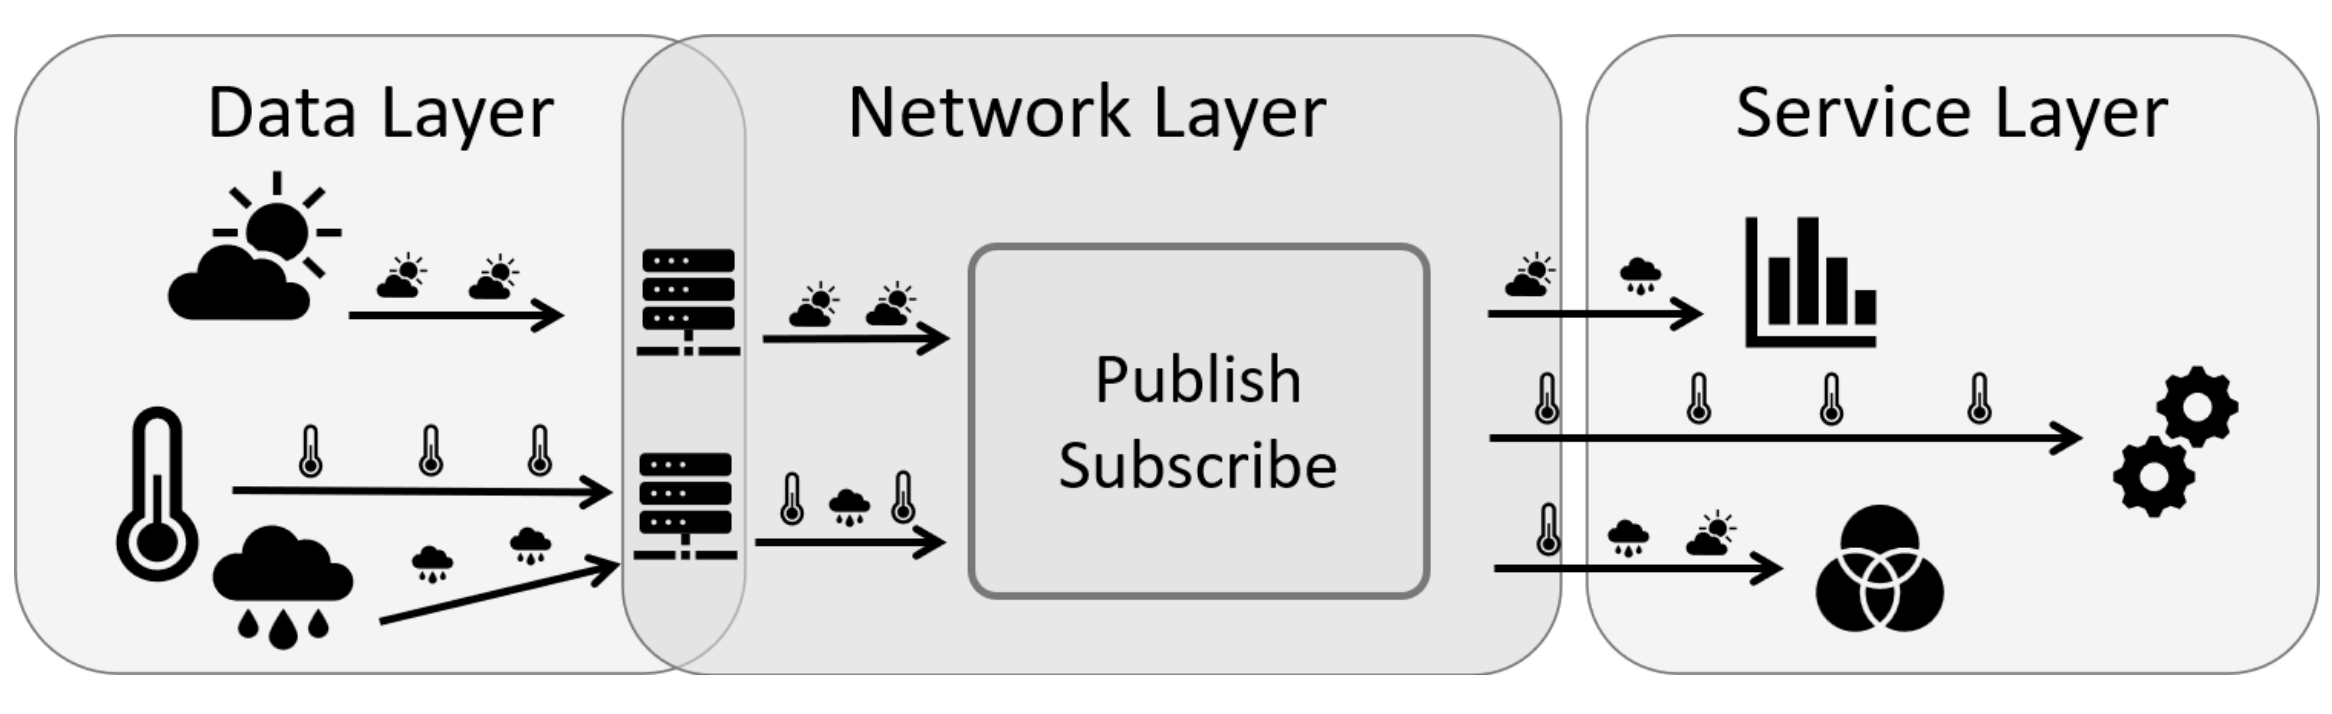
\includegraphics[width=\textwidth]{images/expose-system-architecture.png}
    \caption{In the data layer (left), a wide variety of environmental data is collected with the help of multiple sensors. These are connected to their citizen-owned local base stations, which manage access rights and forward collected data to subscribed services (right) via the decentralized publish-subscribe in the network layer (center).}
    \label{fig:system-architecture-overview} %todo: create graphic of the 4 layers instead
\end{figure}

% Todo: potentially write more about SANE and data marts etc.

\subsection{Architecture Layers}

\subsubsection{Sensing Layer}

% todo: take a closer look at sensing layer with challenges like sensor placement, uncertainty etc.

The goal for the sensing layer is to monitor the surrounding environment and capture key data for further analysis and decision making. It consists of many different types of physical and virtual sensors. The first group of sensors are the physical sensors, which are placed directly inside the environment. Wireless sensor networks (WSN)~\cite{dargie2010fundamentals} have seen a lot of attention for many different applications such as `military sensing, physical security, air traffic control, traffic surveillance, video surveillance, industrial and manufacturing automation, distributed robotics, environment monitoring, and building and structures monitoring'~\cite{chong2003sensor}. The challenges for WSNs primarily depend among other things on the deployment. An ad-hoc WSN has energy and bandwidth contraints due to the usage of batteries as power sources.
In contrast, sensors that are permanetly installed, either stationary or on a moving target, and connected to a constant power source don't have this constraints. This approach could be used for smart cities to reduce waste and guarantee representative measurements via correct sensor placement. In the case of stationary sensor networks though, the initial deployment and following maintenance cost can be substantial~\cite{chapman2015birmingham}.\\
In recent years, low-cost sensors (LCS) in combination with sensor networks have enabled fine-granular real-time monitoring of urban environments~\cite{grimmond2006progress, rundel2009environmental}, although the quality of individual low-cost sensors can be questionable~\cite{castell2017can}. In general, LCSs can improve data availibility and support analysis, but do not substitute well-calibrated reference instrumentation~\cite{lewis2018low}.
% could also discuss low cost sensors

\subsubsection{Stationary Sensor Types}
There are many different types of environmental features that can be measured directly inside an urban area. The types of measurements that can be observed are among others: air temperature, humidity, atmospheric pressure, reactive gaseous air pollutant (CO, NOx, O$_3$, SO$_2$), particulate matter (PM), greenhouse gases (CO$_2$, CH$_4$), percipitation, solar radiation, wind speed and direction, anthropogenic heat, noise, sky-view factor, heat fluxes and many more. % Todo: Soil
Correlations between these features can vary greatly based on surrounding factors. In order to better understand these correlations, many empirical studies have studied the influence of meteological factors on features such as PM~\cite{tai2010correlations}. Additionally, many fields of statistics have specialised on topics such as statistics in climatology~\cite{von2002statistical}, geostatistics~\cite{trangmar1986application} and more.\\
All sensor readings that are taken by physical sensors are singular data points. Additionally to the type of measurement taken and the actual value observed, physical sensor readings include the physical location of the sensor, e.g. latitude, longitude and altitude, the type of sensor used to take the measurement, and the sampling rate. For air temperature, the sampling rate could be an average temperature measured over five minutes, whereas percipitation might be measured by collecting rain for certain periods of time and then measuring the amount of rain collected. The sensor type is important, as different types of sensors can produce different qualities of measurements, e.g. LCS compared to callibrated reference-grade high cost sensors, and perform better or worse based on the meteological conditions, e.g. worse performance at low temperatures, high humidity etc. Due to the placement directly inside the environment, (near) real-time observation and high temporal resolution are generelly possible, but might be influenced by factors such as network availability. The spatial resolution highly depends on the number of sensors deployed and the correct placement of the sensors. The correct placement has a direct influence on the footprint of the sensor~\cite{leclerc2014footprints} and the representativness of the measurement taken for the underlying and surrounding area~\cite{oke2006guideline}.\\
One downside of the placement directly in the environment the sensors are observing, is the exposure to environmental influences such as heat, humidity, or pollution, that can decrease the lifetime of a sensor and may require more frequent maintenance or replacement.

% Todo: list of sensors with downsides

- discussion premium vs low-cost sensors
- discussion static data incorporation -> NDVI from geoportal via data management layer

- P2,5: highly depends on air flows
- humidity: needs to be replaced more often due to pollution
- temperature

\subsubsection{Mobile Sensor Types}

% describe how mobile sensors can be used to complement stationary sensors
- mobile Windmessungen mit einem SODAR - einem akustischen Windmesssystem -, Vergleichsmessungen an einer stationären Messstelle auf
- Profilmessfahrten



\subsubsection{Modelling of the Sensing Layer}

A model is an abstraction of the real world that helps us analyse and understand complex problems. In the context of UHI detection, we can use model climate on a bigger scale, or the micro-slimate inside a city, to better understand and capture influences. In this work, we focus on ...\\
% Todo
One major consideration in this context, what type of data is used to validate and train the ML models. The options in this case are either climate models which simulate data, or capturing/collecting real-world data. Due to the complexity and limitations of simulation, this work only focuses on collecting real-world data.
% Todo


\subsubsection{Data Transportation Layer}

\subsubsection{Data Management Layer}

\subsubsection{Application Layer}

The application layer contains services which utilize data provided by the data management layer to provide services for the city and its citizens. As part of this layer, services could be build that aggregate data streams coming from the data management layer and use ML to improve the data quality by detecting outliers, reducing bias, interpolating missing data etc. The improved data could then be published and other services that would otherwiese rely on the raw data streams and potentially need to implement their own outlier detection or interpolation of missing data techniques, instead simply subscribe to the externally managed service. This could lower the barrier to entry for developers with less available resources, financially or domain-knowledge wise, and generelly allow developers/service providers to allocate their resources to other areas like user experience (UX) and usability compared to the maintenance of complex ML-based services.\\
In the context of this work, we focus on the topic of UHI detection. In this context, there could be a UHI detection service that ingests real-time data streams from the data management layer and notify citizens if an UHI is detected in or predicted for a particular urban area. As the main challenge for UHI detection lies, next to the definition of urban and rural reference areas, on the gathering of a comprehensive temperature map that allow UHI detection algorithms to work, in this work we primarily focus on creating and evaluating an air temperature map service, that enables the detection of CUHIs and could also be used as a foundation for other services in a smart city, like plant watering systems, smart healthcare and more.

% Todo: not sure if needed
\subsection{Smart City Case Studies}
\label{sec: smart city case studies}
% get from data management list...

Many european cities, like Amsterdam, Barcelona, London and Stockholm, have developed their own smart city strategies and platforms. In the following, we take a closer look at the steps each city has taken:\\
\\
\textbf{Barcelona, Spain}: Barcelona operates the `Sentilo' platform~\footnote{\url{http://www.sentilo.io/}}, an open-source smart city platform that aims to break down informatioal silos inside the city to provide unified access to the data available. It currently contains more than 27.000 sensors~\footnote{\url{http://connecta.bcn.cat/connecta-catalog-web/stats/} (\textit{Accessed: 23.03.2023})}. It offers a modular and extensible architecture, high performance and scalability, alerts, stats, triggers, a simple REST API to send and receive sensor data, and is cross-platform by being build with Java, Redis and MongoDB.\\
%Todo: move to section with case studies
\\
\textbf{Amsterdam, Netherlands}: Amsterdam utilizes sensors to run an extensive smart lighting system, that\\
\\
\textbf{London, England}: More infos\\
\\
\textbf{Stockholm, Sweden}: More infos\\
\\
More honorable mentions from outside the EU:\\
\\
\textbf{Singapore}: more infos\\
\\
\textbf{San Fransico, US}: more infos\\

\section{Sensing Applications}

\subsection{Remote Sensing}

In comparison to stationary sensors that are installed directly in the environment they are observing, remote sensing describes the process of observing a target environment from afar~\cite{campbell2011introduction}. In climatology, remote sensing is used to collect meteological data via satellites, planes or ballons by either capturing image data, that can be used to identify things like cloud and land coverage, by measuring passive radiation, or by actively sending out microwaves or using LIDAR to detect features such as surface temperature, e.g. LST data. Remote sensing comes with its own set of advantages and challenges.\\
The major upside of sensors moving way above ground is the high spatial coverage, that allows for meso- and planetary-scale anaylsis of weather phenomena. Another upside is the great data availibility, as many satellite providers, such as ESA..., publish their satellite data. This creates many research opportunities, and many services directly rely on these measurements (todo list).\\ % gridded data
% remote sensing challenges
Remote sensing also comes with some downsides. The primary downside is the low spatio-temporal resolutions. Weather satellites usually are not orbit-stationary and move around earth on a predetermined orbit. As a consequence, satellites only pass over each individual area a couple times a day, making real-time applications for currently unobserved areas impossible. Additinally, the spatial resolution can be too low for micro-/local-scale analysis, with typical LST resolution spanning from 1 km$^{2}$ to tens or even hundreds of km$^{2}$ per data point/grid field. In the atmosphere, there is also a lot of environmental noise, like radiation, that can have a negative influence on the measurement accuracy. Another disturbing factor can be clouds or other types of particles like rain, that absorb radiation/microwaves sent from the sensors, traditionally making measuring under cloudy/rainy conditions either impossible (example) or less accurate (example), by instead relying on outgoing radiation from the surface. These restrictions highly depend on the sensor used, as different sensors use different 
sensors use different technologies, e.g. microwaves with different wave lengths or higher resolution sensors.



% todo: potentially more to the downsides of each sensor type / overview of types of satellites

\section{Interpolation of Missing Data}

% First overview: interpolation techniques/history
% - foundation in statistics
% - adaptation for specific research areas (focus on temperature related research in this thesis)
%     - geostatistics (Krigin) -> probabilities need to be known
%         - climate research (macro) -> global warming, temperature trends
%         - urban climate research (micro) -> heat islands, polution
%     - ML approaches (deep learning, random forests etc.)
%         - list some approaches

In the context of urban environments, there are many measurements such as surface temperature, which are measured by sensors that have certain weaknesses. In the case of LST data collection, clouds play a mayor part and prevent surface temperature to be measured. In many LST data-sets (ref), measurements for cloud areas are simply defined as having no value. As many applications and algorithms need continous input data to work as expected, in this work we take a look on how interpolation, especially with the help of ML, can help solve this problem. In the context of LST data, this could mean interpolating the missing data either based on surrounding data (cite) or by integrating many different features such as air temperature, humidity, heat flux etc. in a ML model (cite).\\
- moving sensors for better spatial coverage into unobserved areas

\subsubsection{Interpolation vs. Extrapolation}

In this work, we focus on interpolation of missing data. Interpolation is the process of calculating/guessing missing values between given values. This could be a missing value in a time-series or a missing cell in a data grid (cite). In contrast, extrapolation is the prediction of values based on previous values, like predicting values based on historic time-series data, es in the case of weather forecasting. Due to time constraints, we only focus on the interpolation part, tho extrapolation could also play an important role in smart cities by predicting UHIs and warning citizens about potential future heat-related risks.

\subsection{Regression Analysis in Statistics}

Fundamentaly, regression analysis has its roots in mathematics, more specifically in the field of statistics.
todo: more

- foundation of other research fields, based in statistics/mathematics

- linear regression (least-squares)
- multiple regression models
- hierachical regression

- special cases
    - piecewise linear regression
    - inverse prediction
    - weighted least squares
    - logistic regression
    - poisson regression

\subsection{Interpolation in Geostatistics}

- spatiotemporal (kriging)
- time series prediction vs interpolation of missing data
- based on GIS 
- pipeline: fit measured data points to grid, interpolate missing squares
downside: cannot find local maximas/minimas

\subsection{Applications for Machine-Learning}

traditional interpolation techniques are simple and usually fast, but lack the ability to adapt to the specific problem at hand.

transition to ML based Interpolation

applications:
- all-in one solution (all features included) -> huge DL model with billions of parameters (ChaptGPT)
    - not feasible in this thesis
- pipeline solution (use ML models incrementally and build upon results)
    - similar to NLP
    - feasible for specific topics
    - bottom-up approach (use ML to increase the amount of available data)

- types of ML utilisation
    - utlier detection
    - classification
    - regression
        - interpolation of missing data
        - prediction of future data
